\section{\system{} Design}
\label{sec:design}

\system{} that provides oblivious content distribution and  
comprises the following components: clients, exit proxies, CDNs, and origin 
servers.  {\em Clients} are the Internet users who use the system to access content
stored on CDN cache nodes; {\em exit proxies} are proxies that obfuscate the requests
and responses retrieved from the CDNs; and the {\em origin servers} are the content
publishers who are customers of the CDNs.  Figure \ref{fig:ocd_overview} shows how
these components interact.  This section discusses the design decisions of \system{}, and what functionality each decision provides.  
We separate design decisions into two parts: 1)~hiding content and 2)~hiding clients.  We also highlight some additional options that the design of 
\system{} allows.

\begin{figure}[t!]
\centering
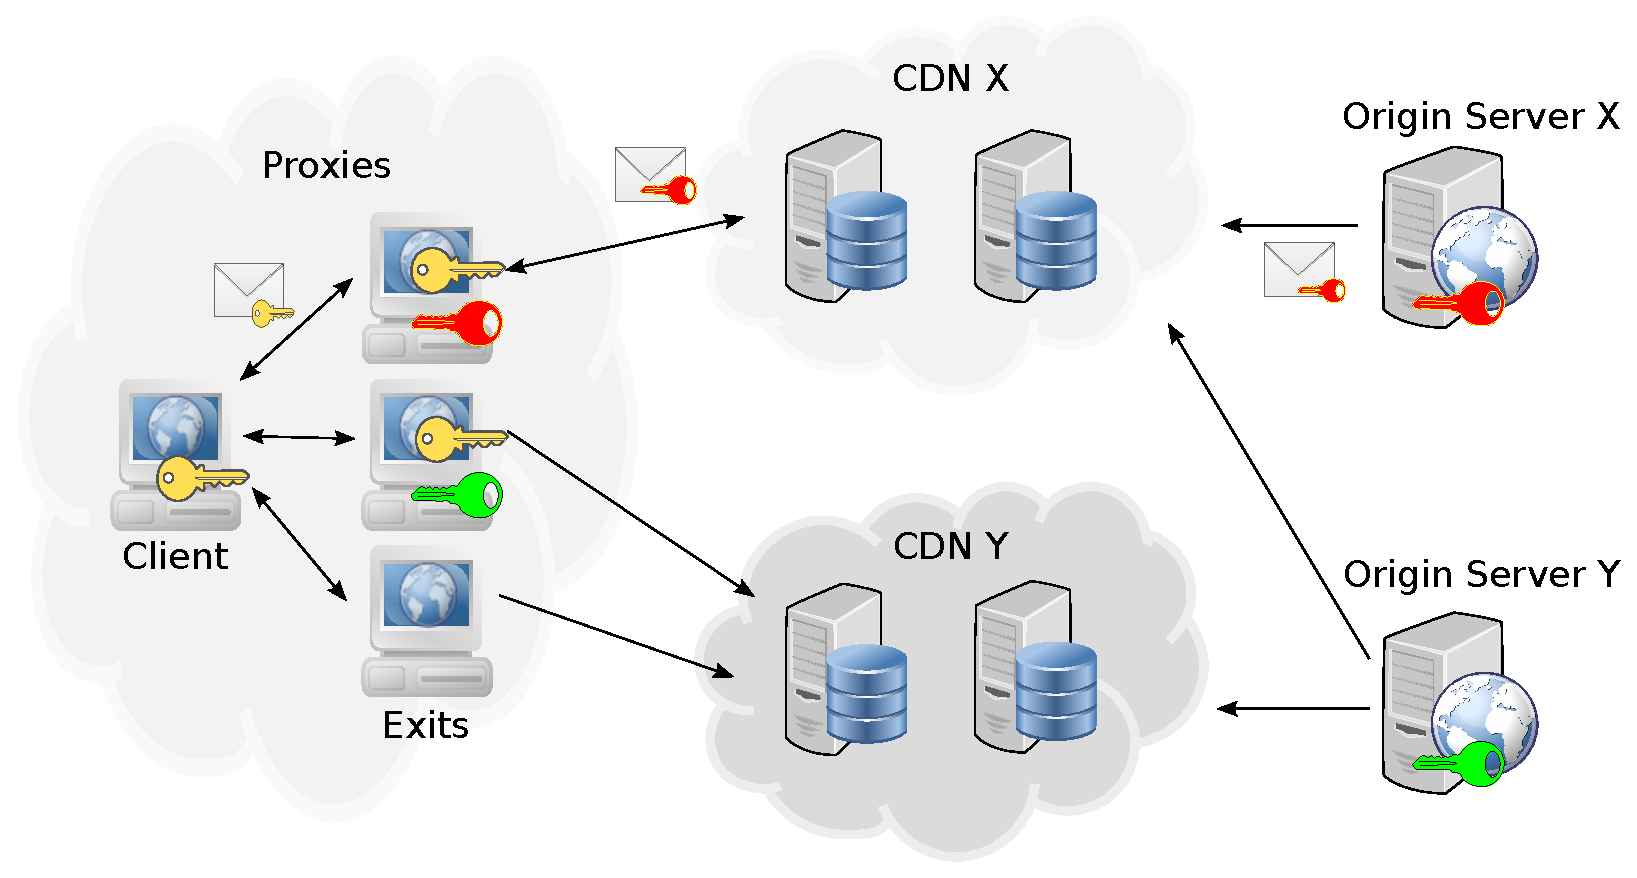
\includegraphics[width=.44\textwidth]{ocdn_overview_new2}
\caption{The relationships between clients, exit proxies, CDNs, and origin servers in 
\system{}.}
\label{fig:ocd_overview}
\end{figure}

\subsection{Hiding Content}
\label{sec:hiding_content}

We start by discussing how the system components communicate and authenticate one another. 
We introduce shared keys between origin servers and exit proxies, how these keys
are stored, how the exit proxies authenticate themselves to origin servers, and how these 
keys are distributed.

%\begin{table}[t!]
%\footnotesize
%\centering
%\begin{tabular}{ l  p{1.9in} } 
% \multicolumn{1}{c}{\bf Design Decision} & \multicolumn{1}{c}{\bf Function} \\
%\hline \hline
% Shared Keys & {Hides content on cache nodes from CDN.} \\
% Consistent Hashing & {Load balance requests across proxies; ensure no proxy can
% control a given URL.} \\
% Self-Certifying Identifiers & {Authenticates exit proxies to origin servers.} \\
% DNS for Key Sharing & {Allows origin server to share shared keys with exit
% proxies.} \\ \hline
%\end{tabular}
%\caption{Design decisions associated with hiding content from a CDN.}
%\label{tab:setup}
%\end{table}

\textbf{Shared Keys.} 
To prevent an adversary from learning information about content and clients, the CDN must not know anything
about the
content that it is caching.  Therefore, the content {\it and} the associated URL
must be obfuscated
before the CDN sees them.  The content can be obfuscated by encrypting it with a
key that is not
known to the CDN.  Because this must be done prior to any caching, the content publisher must 
generate a shared key $k$ to encrypt the content with. Encrypting the content alone does not 
hide all information about content from the CDN; the content identifier, or URL, must also be obfuscated, otherwise the 
CDN can still reveal information about which clients accessed which URLs (which is indicative 
of the content).  The obfuscated URL should be fixed and relatively
small; 
these requirements reduce storage requirements and prevent the adversary from guessing
the
URL based on the length of the obfuscated URL.  Unfortunately, using a simple hash allows an 
attacker to guess the content identifier by hashing guesses and comparing with 
the hashes stored in the CDNs caches.  To prevent this attack, the content publisher incorporates the use 
of the shared key $k$ into the hash of the URL by using a hash-based message authentication code 
(HMAC).  Additionally, if the domain supports HTTPS requests, then the content publisher must 
also encrypt the associated certificate with the same key $k$.

The encrypted content and corresponding HMAC are sent to the CDN\footnote{Most CDNs
allow the publisher to
decide on a push or pull model, but \system{} is compatible with either approach.}
and stored in
its caches.  The content publisher then shares the key $k$ with an exit proxy. 
This key allows the 
exit proxy to request encrypted content on behalf of clients by computing the HMAC on the URL.  

\textbf{Consistent Hashing.}
Each exit proxy stores a mapping of URLs to their associated shared key $k$; for example, if 
an origin server has shared key $k$ and publishes a web page {\tt www.foo.com}, then an exit 
proxy will store the mapping of {\tt www.foo.com} to $k$.  The set of exit proxies jointly compute a distributed hash table where the key is the URL ({\tt www.foo.com}) and the value is the 
shared key ($k$).  To assign (key,value) pairs to exit proxies, \system{} uses consistent 
hashing~\cite{karger1997consistent,lewin1998consistent}.  Consistent hashing uses a hash function $H(.)$
to generate identifiers for both exit proxies and for URLs; the identifiers are $H(exit\_ID)$ and $H(URL)$. 
We discuss what $exit\_ID$ is in the next section on Self-Certifying Identifiers.  After the hashes are 
computed, then they are mapped to a point on an identifier circle (modulo 2$^{m}$, where $m$ is the length of 
identifier in bits); each URL ($H(URL)$) on the circle is assigned to the first exit proxy ($H(exit\_ID)$) that 
is equal to or follows $H(URL)$ on the circle.  This hashing method is used in \system{} because it provides: 
1)~an evenly distributed mapping of URLs to shared keys among the exit proxies,
2)~a way to prevent an exit 
proxy from choosing which URL it wishes to be responsible for, and 3) a relatively small amount 
of (key,values) to be moved when a new exit proxy is established (or removed).  

\textbf{Self-Certifying Identifiers.} Consistent hashing uses identifiers for both the URLs and 
the exit proxies.  While the identifiers for URLs are straightforward ($H(URL)$), the identifiers for exit 
proxies must provide more information; an exit proxy identifier must be able to prove to an origin server that 
it is the exit proxy that is responsible for the associated URL.  If this validation was not part of \system{}, 
then any (potentially malicious) exit proxy could request the shared key $k$ from any or all origin servers.  To 
prevent a malicious exit proxy from learning any shared key $k$, the proxy must be identified by a self-certifying 
identifer.  This technique was first introduced in a self-certifying file system~\cite{mazieres2000self}; it allows
for other entities (such as origin servers) to certify the exit proxy solely based on its identifier.  The format 
of this identifier ($exit\_ID$) is {\tt IP:hostID}, where {\tt IP} is the exit proxy's IP address and {\tt hostID} 
is a hash of the exit proxy's public key.  A malicious exit proxy cannot \textit{choose} where on the consistent 
hashing ring it sits because it cannot frequently change and re-hash its own IP address (whereas it could re-generate 
a new public key).\footnote{While a malicious exit proxy cannot specifically choose its location on the hashing ring, it 
could recompute a public key until it finds a certain location on the hashing ring.  This is limited by the fact that 
the exit proxy's IP address is part of its identifier, and we assume that the adversary running the exit proxy cannot 
change IP addresses to a value of his choice or in a frequent manner.  A potential attack that an adversary can execute 
on a DHT using a consistent hashing scheme is a Sybil attack, where the adversary runs {\it many} exit proxies to hopefully 
place himself in his desired location on the hashing ring.  We describe countermeasures to a Sybil attack in Section 
\ref{sec:sec}.} When an exit proxy is requesting the shared key $k$ from an origin server, 
it sends its identifier and its public key to the origin server.  The origin server
can then hash the exit proxy's 
public key and verify it against the {\tt hostID}; this action serves as a proof
of the exit proxy's position in the consistent hashing
circle, and thus prevents a proxy from lying about where it lies on the ring (and subsequently lying about which 
URL's shared key it is responsible for).  Note that this $exit\_ID$ is used on the consistent hashing circle as $H(IP):H(hostID)$; the 
$exit\_ID$ must be the same length as $H(URL)$, so the $exit\_ID$ consists of the first half of the bits of $H(IP)$ concatenated 
with the first half of the bits of $H(hostID)$.

\textbf{DNS for Key Distribution.}
We have discussed how shared keys are generated, used, and stored, and here we describe how they are shared.  As previously 
stated, the origin servers generate shared keys and must share them with the (correct) exit proxies.  \system{} uses DNS
to do so.  To retrieve a shared key $k$, an exit proxy sends a DNS query to the origin server's authoritative DNS, and 
it includes its identifier, $exit\_ID$, and its public key in the {\tt Additional Info} section of the query.  The 
authoritative DNS for the origin server validates the exit proxy by hashing the public key and comparing it to the 
second part of $exit\_ID$, and verifying that the exit proxy is responsible for its URL based on the consistent 
hashing circle.  If the verification is successful, then the authoritative DNS sends the shared key $k$ encrypted 
under the exit proxy's public key, \{$k$\}$_{PK_{exit}}$ in the SRV record of the DNS response.  The exit proxy 
extracts $k$ by decrypting with its private key, and stores it in its hash table.

%\begin{table}[t!]
%\footnotesize
%\centering
%\begin{tabular}{ l  p{1.9in} } 
% \multicolumn{1}{c}{\bf Design Decision} & \multicolumn{1}{c}{\bf Function} \\
%\hline \hline
%Spoofed Source Routes & {Hides origin of client request from other
% clients, exit proxies, and CDN.} \\
% Session Keys & {Hides URL and response from other clients.} \\
% Multicast Response & {Allows CDN to return content directly to client without knowing
% the client that requested the content.} \\
% \hline
%\end{tabular}
%\caption{The design decisions associated with content requests and responses, and what these 
%decisions provide.}
%\label{tab:request_response}
%\end{table}

\subsection{Hiding Clients}
\label{sec:hiding_clients}
We make additional design choices that concern the requests that clients initiate
and the responses they receive. We 
introduce session keys, how requests are routed from clients to exit proxies, and how responses 
are routed from exit proxies back to the original client.

\textbf{Request Routing with Potentially Spoofed Source Routes.}
As previously described, exit proxies query the CDN on behalf of clients, but the
exit proxy
should not be able to learn which client sent which request.  This obfuscation is
accomplished by routing requests through
a series of other clients.  Each client runs a proxy and is
also a peer in this system; this 
peer-to-peer system of clients borrows the 
protocols used for clients joining, leaving, and learning about other clients from
the vast literature on peer-to-peer systems~\cite{monnerat2006d1ht,risson2006stable,zhu2005efficient,gupta2003kelips,lesniewski2008sybil,leong2004achieving}. A client routes a request through
her peers by using source routing; when the client generates a request, it also
generates a source route, which includes
the addresses of a set of her peers.  The last hop in the source route is the exit proxy that is responsible for the 
shared key $k$ associated with the URL in her request.  The client determines the correct exit proxy by looking up a locally-held URL-proxy map (which is retrieved from a central system that keeps the mapping of URLs to exit proxies).  
It appends this source route to its request and forwards it to the next peer
in the route.  When a peer receives
a request, she simply forwards it on to the next peer; this continues until the last hop in the source route, which 
is an exit proxy. 

To obscure the client that initiated the request, \system{}
allows each client to spoof source routes; specifically, a client can prepend
other peers in the route before it initiates a request.  For example, a client
with identity {\it C} could generate a route to exit proxy {\it E} that looks
like $C \rightarrow G \rightarrow F \rightarrow E$ and can further obfuscate
the source of the route by prepending additional clients to the beginning of
the route as follows: $D \rightarrow A \rightarrow C \rightarrow G \rightarrow
F \rightarrow E$. Neither {\it G}, {\it F}, nor {\it E} know who the original requestor was; from {\it E}'s point of 
view, the original requestor could have been {\it D}, {\it A}, {\it C}, {\it G},
or {\it F}.  Recall from Section \ref{sec:attacker} that our threat model does not 
include a global passive adversary, and therefore do not prevent an adversary with those capabilities 
from learning which client issued the request; \system{} does prevent an adversary that is running a 
client and/or exit proxy from identifying which client issued the request. Using a sequence of 
peers, or even just knowing that a client {\it can} use a series of peers, hides
the identity of the client 
from other clients, exit proxies, and the CDN. 

Spoofed source routes offer a tradeoff between privacy and performance. Clients interested in prioritizing performance can choose to send requests directly to the exit proxy. In such a case, the exit proxy will know the client's identity, but the CDN will not. For more privacy, the client can forward a request through a set of clients between it and the exit proxy. Lastly, the client could {\it only} prepend other clients' identifiers but simply forward the request {\em directly} to the exit proxy; this action provides the same performance benefit as the first mode, but still offers some additional privacy benefits. Although the last option would appear to strike the optimal balance between privacy and performance, it cannot be the only option because the exit proxy would always know that the true client is the previous hop in the source route. % These modes of operation provide clients with different ways to use the system both based on their privacy preferences and the type of content they are requesting.


\textbf{Session Keys for Request and Response Confidentiality.}
In addition to shared keys between origin servers and exit proxies, \system{} uses session keys shared 
between clients and exit proxies.  Session keys provide confidentiality of the requested URL and the 
response.  When the client generates a request, it generates a session key $skey$.
and encrypts 
the URL in her request with this key, which provides \{URL\}$_{skey}$.  The client
must also share this session key
with the exit proxy, so that the exit proxy can learn the plaintext URL and subsequently compute the HMAC to 
query the CDN.  The client encrypts the session key with the exit proxy's public key, result in \{skey\}$_{PK_{exit}}$, 
and appends this value as an additional header on the request.  Because her request
could be forwarded through 
a set of client peers, this hides the URL of the request from other clients.

When an exit proxy receives a request from a client, it first extracts the session
key $skey$ by decrypting it with 
his private key, and then he decrypts the URL with the session key.  This operation
yields the original plaintext
URL. Using the shared key $k$ from the origin server, it can then compute
HMAC$_k$(URL) and forward the request 
to the CDN.  Upon receiving a response from the CDN, the exit proxy then decrypts
the content with the shared key $k$, and
encrypts the content with the session key $skey$ before sending it to the client.
When it receives the encrypted response, 
the client can then decrypt it using $skey$.

\textbf{Multicast Responses.}
Using session keys allows for a performance optimization in sending responses back to clients.  Instead of sending 
the encrypted response from the exit proxy back to the client via the set of peers used in the source route, the exit 
proxy can send it in a multicast manner to all clients that were on the source route.  The only client that knows $skey$ 
is the true client that originated the request, therefore none of the other clients can interpret the response, and it reduces the 
latency for sending the response to the client.  

%\subsection{Incentives for Running \system{}}
%As described in Sections \ref{sec:hiding_content} and \ref{sec:hiding_clients}, \system{} relies 
%on the use of a system of proxies.  These include: 1) client proxies, and 2) exit proxies.  For a client 
%to join the system, they must also run client proxy on his/her machine.  On the other hand, there is no 
%requirement for a client, organization, or company to run an exit proxy; despite this lack of requirement, we 
%believe that both clients and companies have enough incentives to run an exit proxy (or multiple exit proxies).  
%Clients benefit from running an exit proxy because it allows \system{} to perform better in terms of both 
%performance and privacy; when there are more exit proxies, then there is less load put on each exit proxy, and there is a smaller
%chance that an attacker has access to most exit proxies.  Companies benefit from running an exit proxy for similar 
%reasons --- performance and privacy ---, but it could help Internet users access their content quicker (assuming they have 
%content cached by the CDN).    

\subsection{Design Alternatives}
While our explanation of the design of \system{} describes a series of proxies that are run by us, but are not 
trusted; here we describe alternative designs regarding the system of proxies.  The system will work with both a closed, 
trusted system of proxies, as well as with an open (untrusted) system of proxies.

{\bf Closed System of Proxies.} While the proxies in \system{} are not trusted, \system{} could 
use a system of closed and trusted proxies.  There are potential groups or organizations that would 
support this type of system, and would be willing (and trusted) to run the exit proxies.  If the exit
proxies were trusted, then parts of the design of \system{} could be simplified; for example, if proxies 
were trusted, then \system{} would not need to hide the identity of clients from the exit proxies, and could 
remove spoofed source routes from the design.  The primary drawback of this approach is finding an organization 
that everyone could trust to run the exit proxies.  

{\bf Open System of Proxies.} In \system{}, exit proxies are not 
trusted with client identities and information, which removes the need to find a universally trustworthy 
organization.  In an alternative approach, \system{} could use a completely open system of proxies that are 
untrusted, which would allow anyone (clients, companies, etc.) to run an exit proxy.  
The addition of an exit proxy follows the protocol in consistent hashing for when a new node 
joins; some keys would be transferred to the new exit proxy, and clients' mapping of 
exit proxies will be updated.  This allows for the load to be split among more proxies and 
increases the geographic diversity of the exit proxies.  

\subsection{Design Enhancements}

We discuss possible enhancements to \system{}'s basic design.

%\textbf{Multiple CDNs.}
%While describing the design decisions that went into \system{}, we referred to a single CDN for 
%simplicity.  In reality, \system{} allows for many CDNs to participate;
%distributing content across
%multiple CDNs could provide additional privacy. Origin servers can also take advantage
%of multiple CDNs.

\textbf{Encoding URLs.}
As described earlier, each URL is obfuscated by using a HMAC and then stored on the CDN.  An adversary 
could potentially correlate a URL's popularity with its access patterns.  To prevent this, \system{} allows 
origin servers to generate multiple different encodings of its URLs, such that HMAC$_k$(enc$_1$(URL)) $\neq$ 
HMAC$_k$(enc$_2$(URL)).  Each origin server could produce $n$ different encodings of popular URLs, such that 
the popularity distribution seen by an adversary is a uniform distribution of URL requests across all URLs.  

\textbf{DHT Replicas.}
Each exit proxy's hash table can be replicated by another (or many other) exit proxies, spreading the burden across multiple proxies. This behavior would provide less load per exit proxy, as well as redundancy in case of failures.  Additionally, 
the CDN can cache the content associated with a given URL at more than one cache
node;
if only one exit proxy is responsible for a given URL's content, then it would likely only be cached at 
cache node closest to the exit proxy.  Having multiple exit proxies responsible for a URL's content 
helps decrease the load on the proxies while maintaining some of the performance benefits of a CDN.

\textbf{Hybrid OCDN/CDN Designs.}
Different origin servers have different needs, and each origin server might 
have different needs for different content.  The design of \system{} allows origin servers
 to publish some of their content on \system{} and some on other CDNs.  
This is useful in a case where some content is more sensitive, while other content needs 
better performance.

\textbf{Pre-Fetch DNS Responses.} 
One way to increase the performance of \system{} is to pre-fetch DNS responses at 
the exit proxies.  This would allow the exit proxy to serve each client request faster 
because it would not have to send as many DNS requests.  Pre-fetching DNS responses would 
not take up a large amount of space, but it also would not be a complete set of all DNS 
responses.  Additionally, if the CDN moves content between cache nodes, then DNS 
response must also change; therefore, the pre-fetched DNS responses should have a lifetime 
that is shorter than the lifetime of the content on a cache node.

%\textbf{Privacy vs. Performance Tradeoffs.}
%There are two different modes that \system{} can operate in, where one provides better 
%performance, and the other provides better privacy.  In the first mode, the client can 
%choose to send a request directly to the exit proxy.  
%
%In this case, the exit proxy might be able to discover the identity of the client,
%but the CDN would still not be able to map a request to the client that made the
%request.
%Alternatively, the client can forward a request
%through a set of peers before it reaches the exit proxy.  In this case, the client
%can 
%prepend other clients' identifiers (as previously described) to make it appear as
%though the request came from
%a different client.  This action further obscures the relationship between the client
%and the request.  As another option, the client could {\it only} prepend
%other clients'identifiers but simply forward
%the request {\em directly} to the exit proxy; this action provides the same performance
%benefit as the first
%mode, but still offers some additional privacy benefits.  Although the last option
%would appear to strike the optimal balance between privacy and performance, it cannot
%be
%the only option because the exit proxy would always know that the true client is the previous hop 
%in the source route.  These modes of operation provide clients with different ways to use 
%the system both based on their privacy preferences and the type of content they are requesting.

